\documentclass{article}
\usepackage{amsmath, amssymb}
\usepackage{graphicx ,caption}
\usepackage[a4paper, total={7in,10in}]{geometry}

\begin{document}
\begin{titlepage}
\begin{center}
\textit{\today}
\vfill
\textbf{\LARGE{Ressources énergétiques}\\\Large{Physique --- Chapitre 14}}\\
\vfill
\large{Ewen Le Bihan\\1eS3}
\end{center}
\end{titlepage}

\section{Ressources énergétiques}
\subsection{Environnement}
Énergie primaire $\neq$ Énergie finale

\subsection{Stockage}
\begin{figure}[htp]
\centering
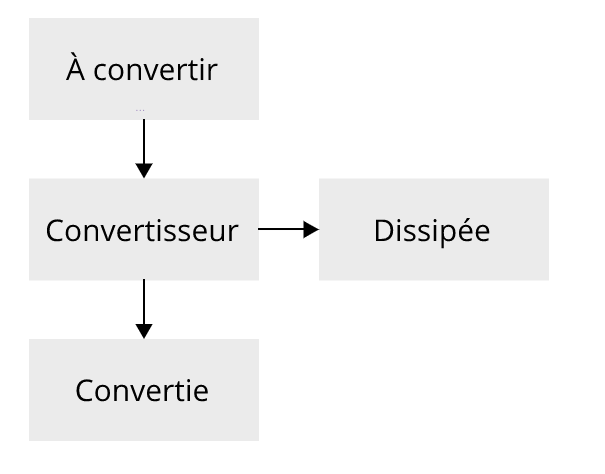
\includegraphics[scale=0.25]{Chap14_Fig1.png}
\caption{Diagramme de conversion d'énergie}
\label{conv}
\end{figure}

\subsection{Puissance \& Énergie}
\begin{flalign*}
E:J &= P \cdot \Delta t\\\\
P &: W\\
\Delta t&: s \;\;\;\text{(Durée de fonctionnement)}
\end{flalign*}
\begin{flalign*}
P:W &= U \cdot I\\\\
U &: V\\
I&:A
\end{flalign*}
\begin{figure}[htp]
\centering
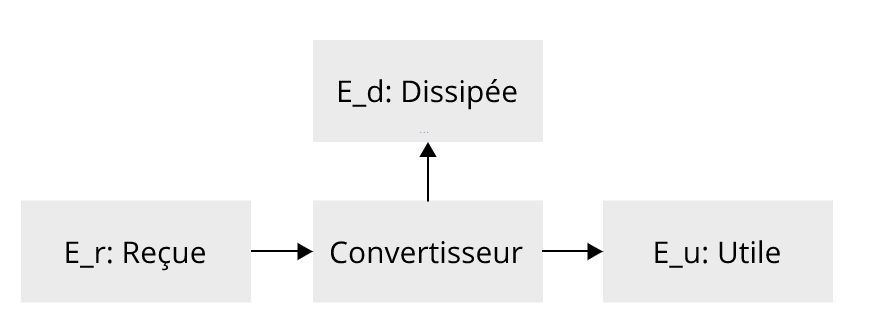
\includegraphics[scale=0.25]{Chap14_Fig2}
\caption{Différentes phases de l'énergie}
\label{phases}
\end{figure}
\subsection{Rendement}
\begin{flalign*}
\eta = \frac{E_u}{E_r}=\frac{E_u}{E_r}\;\;\;\text{avec}\; \eta \in [0;1]
\end{flalign*}
\subsection{Effet joule}
Conducteur ohmique:
Électrique $\to$ Thermique + Rayonnement\\
Peut être génant (ordi, télé, console,...) ou bénéfique (radiateur, bouilloire,...)
\subsection{Equation de caractéristique}
\begin{tabular}{l|l}
	Pile & $U_{PN}=E-r \cdot I$\\
	\hline
	Conducteur ohmique & $U_{AB}=r \cdot I$
\end{tabular}
\\\\
La force éléctromotrice $E$ d'un gén. : Tension $\oplus$ mesurée en circuit ouvert\\
r := résistance interne de la pile
\end{document}